\section{Experimental results}
\label{sec:results}

  We have conducted a set of experiments with the framework described above.
  The main goals of these experiments are (i) to assess the applicability and scalability of model checking for computing WCET estimation for embedded control systems; and (ii) to evaluate the impact of the branch prediction policy on the WCET.

  %We have conducted experiments to evaluate if model-checking is fit to
  %perform precise WCET analyses on model simulating the behaviour of complex
  %architectures for embedded control systems.
  %To do so we use UPPAAL which outputs the following information for each model:
  %i) the number of states explored; ii) the CPU time used; iii) memory used.
  
% Currently, some limitations remain. First of all, the computed branches as
% found in the {\texttt{\small switch ... case}} control structure are not taken
% into account. Similarly, function calls via pointers and recursive calls can
% not be used. Finally, BEST can not currently manage slices where the
% instructions are dependent on each other by local variables located on the
% stack. This last point will be addressed in the future.
  
  We used the Mälardalen WCET benchmarks~\cite{Gustafsson:WCET2010:Benchmarks}
  to generate the programs. We excluded certain programs to account for
  the current limitations of our framework: 
  \begin{enumerate*}[(i)]
    \item TAs are not fit to model recursive programs;
    \item our model of the architecture does not manage floating point
      arithmetic instructions;
    \item BEST does not manage binary executables with indirect branch
      instructions other than function return instructions (\textsl{i.e.} 
      switch-case statements and function pointers);
    \item BEST does not manage slices where instructions depend each others through local
      variables located on the program stack. This point will be addressed in
      the future.
  \end{enumerate*}

  

  %% \begin{table}
  %%   \centering
  %%   \caption{Impact of the branch prediction policy (cf. section
  %%     \ref{sec:architecture:dybrpred}) on the WCET and on the
  %%     complexity of the system. Data in column $x$ vs. $y$ is computed by
  %%     $(x - y)/y$. For instance BTFN vs. AN for bs-O1 means the WCET decreases by 0.95\% and the number of states decreases by 1.87\% when using the BTFN policy instead of the AN policy.}
  %%   \label{tab:policy_impact}
  %%   \small
  %%   \resizebox{\textwidth}{!}{%
\begin{tabular}{|l|r|r|r|r|r|r|}

    \hline
    \multirow{2}{*}{Program} & \multicolumn{2}{|c|}{BTFN vs. AN} & \multicolumn{2}{|c|}{BTFN+BTB vs. AN} &\multicolumn{2}{|c|}{BTFN+BTB vs. BTFN}
    \tabularnewline\cline{2-7}
    
    & \multicolumn{1}{|p{1.5cm}|}{\centering WCET} & \multicolumn{1}{|p{1.5cm}|}{\centering States} & \multicolumn{1}{|p{1.5cm}|}{\centering WCET} & \multicolumn{1}{|p{1.5cm}|}{\centering States} & \multicolumn{1}{|p{1.5cm}|}{\centering WCET} & \multicolumn{1}{|p{1.5cm}|}{\centering States}
    \tabularnewline\hline\hline


bs-O1 & -0,95 \% & -1,87 \% & -3,17 \% & -3,07 \% & -2,24 \% & -1,22 \%
\tabularnewline\hline

bs-O2 & -2,12 \% & -2,43 \% & 0,00 \% & -1,99 \% & 2,16 \% & 0,45 \%
\tabularnewline\hline

bsort100-O1 & -4,40 \% & -5,22 \% & -7,15 \% & -34,70 \% & -2,88 \% & -31,11 \%
\tabularnewline\hline

bsort100-O2 & -1,80 \% & -3,96 \% & -3,65 \% & -32,65 \% & -1,89 \% & -29,87 \%
\tabularnewline\hline

cnt-O2 & -2,59 \% & -2,35 \% & -2,19 \% & -27,27 \% & 0,42 \% & -25,52 \%
\tabularnewline\hline

crc-O1 & -6,57 \% & -7,95 \% & -10,79 \% & -13,89 \% & -4,52 \% & -6,45 \%
\tabularnewline\hline

crc-O2 & -6,18 \% & -7,79 \% & -6,17 \% & -14,37 \% & 0,01 \% & -7,13 \%
\tabularnewline\hline

expint-O1 & -7,16 \% & -7,76 \% & -15,63 \% & -17,56 \% & -9,12 \% & -10,63 \%
\tabularnewline\hline

expint-O2 & -7,34 \% & -7,36 \% & -7,28 \% & -7,28 \% & 0,07 \% & 0,08 \%
\tabularnewline\hline

fdct-O1 & -0,95 \% & -0,09 \% & -0,02 \% & -2,84 \% & 0,93 \% & -2,76 \%
\tabularnewline\hline

fdct-O2 & -0,79 \% & -0,08 \% & 0,00 \% & -2,88 \% & 0,80 \% & -2,80 \%
\tabularnewline\hline

fibcall-O1 & -6,60 \% & -9,37 \% & -7,58 \% & -9,16 \% & -1,05 \% & 0,23 \%
\tabularnewline\hline

fibcall-O2 & -14,01 \% & -15,23 \% & -14,01 \% & -15,23 \% & 0,00 \% & 0,00 \%
\tabularnewline\hline

fir-O1 & -3,23 \% & -3,01 \% & -3,43 \% & -29,10 \% & -0,21 \% & -26,89 \%
\tabularnewline\hline

fir-O2 & -3,36 \% & -3,22 \% & -3,35 \% & -30,34 \% & 0,01 \% & -28,03 \%
\tabularnewline\hline

insertsort-O2 & -1,53 \% & 1,64 \% & -1,47 \% & -15,35 \% & 0,06 \% & -16,72 \%
\tabularnewline\hline

janne\_complex-O1 & -2,93 \% & -4,49 \% & -7,18 \% & -10,64 \% & -4,38 \% & -6,44 \%
\tabularnewline\hline

janne\_complex-O2 & 3,23 \% & -0,17 \% & 2,90 \% & -0,67 \% & -0,31 \% & -0,51 \%
\tabularnewline\hline

jfdctint-O1 & -0,07 \% & -0,92 \% & 0,54 \% & -11,47 \% & 0,61 \% & -10,65 \%
\tabularnewline\hline

jfdctint-O2 & -0,61 \% & -0,89 \% & 0,30 \% & -11,16 \% & 0,92 \% & -10,37 \%
\tabularnewline\hline

ns-O1 & -2,67 \% & -2,80 \% & -6,87 \% & -25,82 \% & -4,32 \% & -23,68 \%
\tabularnewline\hline

ns-O2 & -4,27 \% & -4,57 \% & -4,32 \% & -30,12 \% & -0,05 \% & -26,78 \%
\tabularnewline\hline

prime-O1 & -10,46 \% & -10,68 \% & -10,63 \% & -10,73 \% & -0,19 \% & -0,06 \%
\tabularnewline\hline

prime-O2 & -10,69 \% & -10,80 \% & -10,71 \% & -10,82 \% & -0,03 \% & -0,03 \%
\tabularnewline\hline

ud-O2 & -0,82 \% & 3,63 \% & -0,29 \% & -9,80 \% & 0,54 \% & -12,96 \%
\tabularnewline\hline

\end{tabular}
}

  %% \end{table}

  %We did not include results for programs compiled using more opitmisation
  %techniques (\texttt{-O3}) because these were not significantly different from
  %results for programs compiled using less opitmisation techniques
  %(\texttt{-O2}).
  
  \begin{table}[ht]
    \centering
    \caption{Consumption of resources by the analysis for the AN prediction policy.}
    \label{tab:resource_consumption_an}
    \vspace{1em}
    \begin{tabular}{|l||r|r|r|r|r|}
                                                                                       \hline
    Program           & States explored  & CPU time (ms) & Memory (KiB) \tabularnewline\hline
                                                                                       \hline
    bs-O1             & 586              & 10            & 12684        \tabularnewline\hline
    bs-O2             & 451              & 0             & 12140        \tabularnewline\hline
    bsort100-O1       & 12457            & 130           & 29192        \tabularnewline\hline
    bsort100-O2       & 11982            & 130           & 27868        \tabularnewline\hline
    cnt-O2            & 11279            & 110           & 30504        \tabularnewline\hline
    crc-O1            & 157612           & 1600          & 550048       \tabularnewline\hline
    crc-O2            & 144653           & 1570          & 494760       \tabularnewline\hline
    expint-O1         & 5967             & 40            & 22236        \tabularnewline\hline
    expint-O2         & 4118             & 40            & 13860        \tabularnewline\hline
    fdct-O1           & 6823             & 50            & 23804        \tabularnewline\hline
    fdct-O2           & 7080             & 50            & 25532        \tabularnewline\hline
    fibcall-O1        & 949              & 10            & 12104        \tabularnewline\hline
    fibcall-O2        & 590              & 0             & 11000        \tabularnewline\hline
    fir-O1            & \bf 728321       & \bf 4770      & \bf 655628   \tabularnewline\hline
    fir-O2            & 692704           & 4430          & 608412       \tabularnewline\hline
    insertsort-O2     & 2995             & 20            & 14116        \tabularnewline\hline
    janne\_complex-O1 & 779              & 10            & 12512        \tabularnewline\hline
    janne\_complex-O2 & 594              & 0             & 12572        \tabularnewline\hline
    jfdctint-O1       & 11121            & 100           & 31636        \tabularnewline\hline
    jfdctint-O2       & 11349            & 100           & 33796        \tabularnewline\hline
    ns-O1             & 32482            & 250           & 44964        \tabularnewline\hline
    ns-O2             & 31229            & 230           & 40276        \tabularnewline\hline
    prime-O1          & 12072            & 80            & 26560        \tabularnewline\hline
    prime-O2          & 12056            & 80            & 25564        \tabularnewline\hline
    ud-O2             & 11305            & 380           & 491300       \tabularnewline\hline
\end{tabular}

  \end{table}
  
  We built the binaries with \textsc{Gcc} $5.3.1$.
  Without optimization, \textsc{Gcc} generates code where local variables are
  loaded from and stored to the stack frame each time they are used.
  Such binary executables can not be processed by the current version of our framework.
  Options \texttt{-O1} and \texttt{-O2} force \textsc{Gcc} to output optimized code that uses registers to load and store local variables.
  Thus we created two versions of each of the 14 Mälardalen benchmarks
  fitting our constraints, except for \texttt{cnt.c}, \texttt{insertsort.c} and
  \texttt{ud.c} which make use of the program stack when compiled with option \texttt{-O1}.
  All in all, we have built 25 binaries and for each one we ran our framework to
  compute its WCET on an Intel Core i7-3770 (4 cores, 3.40GHz) with 8GiB of RAM running Debian 9 (64-bit, Linux 4.9).
  Each time, we also collected the number of explored states, the time taken by UPPAAL to perform the exploration, and the amount of memory used.
  The results are summarized in table \ref{tab:resource_consumption_an} and
  figure \ref{fig:ratios}.
  
  Table \ref{tab:resource_consumption_an} displays raw data from UPPAAL for
  models implementing the static always not taken branch prediction policy (AN) which is the worst wrt. resource consumption during the analysis. 
  The worst case for each column is highlighted in bold.
  It is obtained for the binary built from the program \texttt{fir.c} compiled with \texttt{-O1}.
  Even in this case, both the analysis time (less than 5s) and the amount of memory used (less than 640MiB) are very reasonable.
  Our conclusion is that model checking seems to be a promising solution to compute WCET for this type of system.
  Further experiments should be performed to identify the limits of the scalability of the approach.

  Figure \ref{fig:ratios} presents the impact of the branch prediction policy on the WCET (figure~\ref{fig:wcet-ratios}) and the state space (figure~\ref{fig:statespace-ratios}).
  Each bar represents the ratio between two policies: BTFN over AN in dark gray, BTFN+BTB over BTFN in light gray, and BTFN+BTB over AN in medium gray.
  For instance the ratio between the WCET computed for program {\tt expint-O1.c} with the policy BTFB+BTB (1944 cycles) and the WCET computed for the same program with the policy AN (2304 cycles) is 84\% (medium gray bar in slot {\tt expint-O1} of figure~\ref{fig:wcet-ratios}).
  When a bar is above 100\%, it means that the numerator policy performs worst than the denominator policy.
  On the contrary, if the bar is below 100\%, it means that it performs better.
  
  Concerning the WCET, we first remark that most ratios are smaller than 100\%.
  It means that branch prediction policies designed to improve the average case also have a positive impact on the WCET.
  Second, we remark that no branch prediction policy dominates the others: for each case, we have at least one bar below the 100\% threshold and one bar above.
  In the context of WCET analysis, it means that there is no worst policy that could be used to always estimate a worst case upper bound.

  Concerning the state space, we remark that adding the BTB to the model of the architecture does not results in an increase of its size.
  On the contrary we note that the average number of states decreases while using a model simulating a more complex behavior. 
  For example, figure \ref{fig:statespace-ratios} shows a decrease of the state space when using BTFN+BTB over AN policies (medium gray bars) up to 35\% (for \texttt{bsort100-O1}), with an average around 15\%.
  A better prediction policy decreases the number of control hazards and thus the number of configurations of the lower stages of the pipeline, thus reducing the size of the state space.
  In addition, we note that the WCET bound and the size of the state space do not always change in the same direction.
  For instance, in the case of \texttt{fdct-O2}, using BTFN+BTB over BTFN (light gray bar) increases the WCET bound (bar above 100\%) but decreases the size of the state space (bar below 100\%).
  Further experiments should be performed to collect lower level events (eg. cache accesses, memory accesses, flushes of the prefetch buffer, etc.) to better understand this type of phenomenon.

  %For example, figure \ref{fig:wcet-ratios} shows a 3\% WCET reduction and figure \ref{fig:statespace-ratios} shows a 30\% state space
  %reduction for \texttt{fir-O2} wrt. BTFN+BTB and AN policies, while
  %\texttt{bs-O1} yeilds a comparable 3\% WCET reduction for a 3\% state space reduction only.

  %Making less incorrect predictions implies making less instruction cache
  %accesses. Indeed, on correct prediction the instructions to be executed next
  %are already in the instruction prefetch buffer while on incorrect prediction
  %the instruction prefetch buffer contains wrongly prefetched instructions.
  %We speculate that less instruction cache accesses results in a smaller state
  %space.
  
  \begin{figure}[h!]
    \centering
    \subfloat[][WCET ratios]
      {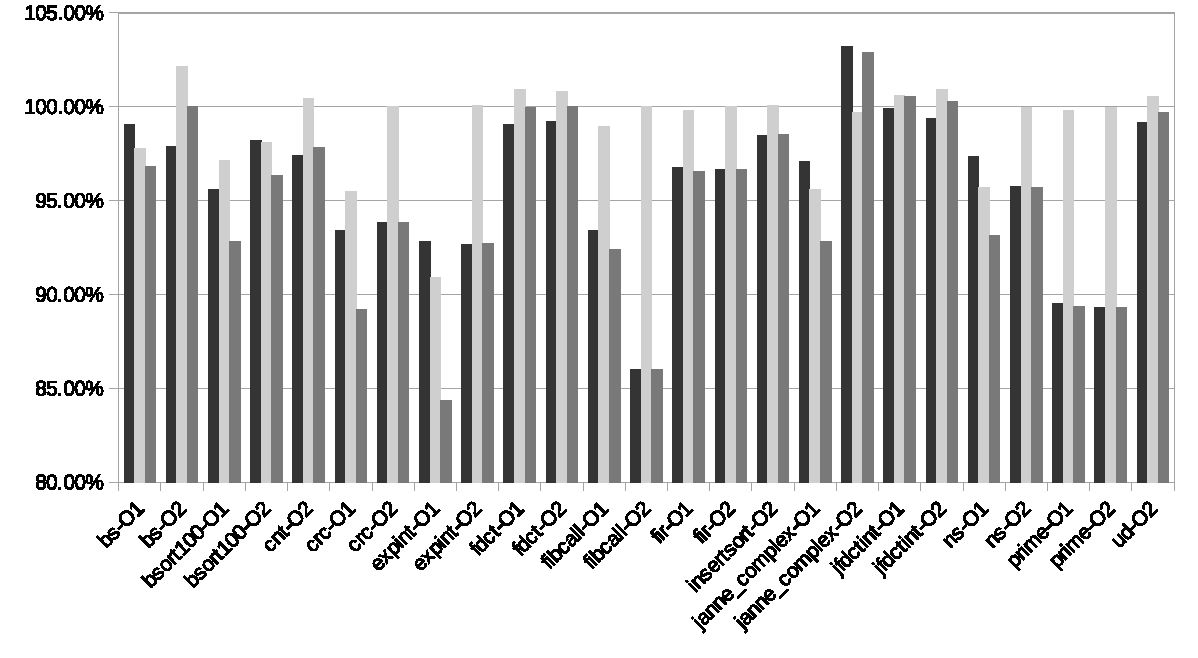
\includegraphics[width=\textwidth]{fig/wcet_ratios_nb.pdf}\label{fig:wcet-ratios}}
    \qquad\qquad       
    \subfloat[][State space ratios]
      {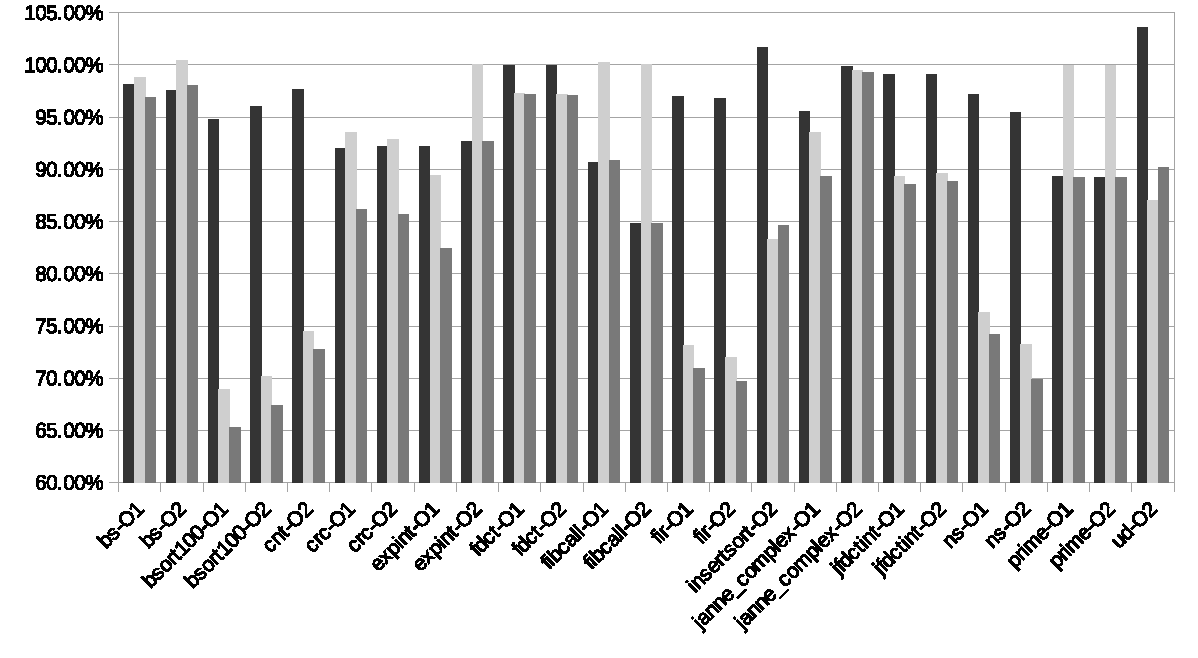
\includegraphics[width=\textwidth]{fig/statespace_ratios_nb.pdf}\label{fig:statespace-ratios}}
    \caption{Impact of the branch prediction policy on the WCET and the size of the state space. Each bar represent the ratio between two policies for a given binary: BTFN over AN in dark gray, BTFN+BTB over BTFN in light gray, BTFN+BTB over AN in medium gray.
      %For example, the WCET of
      %\texttt{expint-O1} using the BTFN+BTB policy (1944 cycles) represent 84\%
      %of its WCET using the AN policy (2304 cycles).
    }
    \label{fig:ratios}
  \end{figure}
  
